%!TEX root = ../booklet.tex
% ^ leave for LaTeXTools build functionality


\begin{metapuzzle}{Fontastic}{Solution}
(FOR STAFF USE ONLY)

The favorite number is \(88\). It is found by interpreting the main Puzzle
solutions as the following fonts and cipher rules.

\begin{itemize}
\item ONE LETTER BEFORE IMPACT
  \begin{itemize}
    \item Font: Impact
    \item Cipher: Rotate all letters back by 1
    \item NVMUJQMFPGFMFWFO \(\Rightarrow\) MULTIPLEOFELEVEN
  \end{itemize}
\item ICE DELIVERY
  \begin{itemize}
    \item Font: Courier
    \item Cipher: Insert the missing letters I
    \item DVDENNESEVENREMAN \(\Rightarrow\) DIVIDENINESEVENREMAIN
  \end{itemize}
\item ALABAMA SHIFTED EAST
  \begin{itemize}
    \item Font: Georgia
    \item Cipher: Move the letters in ALABAMA left by 1
    \item UABNDNAT \(\Rightarrow\) ABUNDANT
  \end{itemize}
\item LAUGH WITHOUT
  \begin{itemize}
    \item Font: Comic Sans
    \item Cipher: Remove the letters in LAUGH
    \item BLEFAOUREGOHNELFAIVUEZGERHO \(\Rightarrow\) BEFOREONEFIVEZERO
  \end{itemize}
\item USE THE UPBEATS
  \begin{itemize}
    \item Font: Syncopate
    \item Cipher: Use every other letter
    \item ETEWDOIOGRITTHSR \(\Rightarrow\) TWOORTHREEDIGITS
  \end{itemize}
\end{itemize}

\(88\) is the only number which is a multiple of \(11\), has a remainder
of \(7\) when divided by \(9\), is abundant (see definition in the rules),
is less than \(150\), and has two or three digits.

\end{metapuzzle}

\newpage


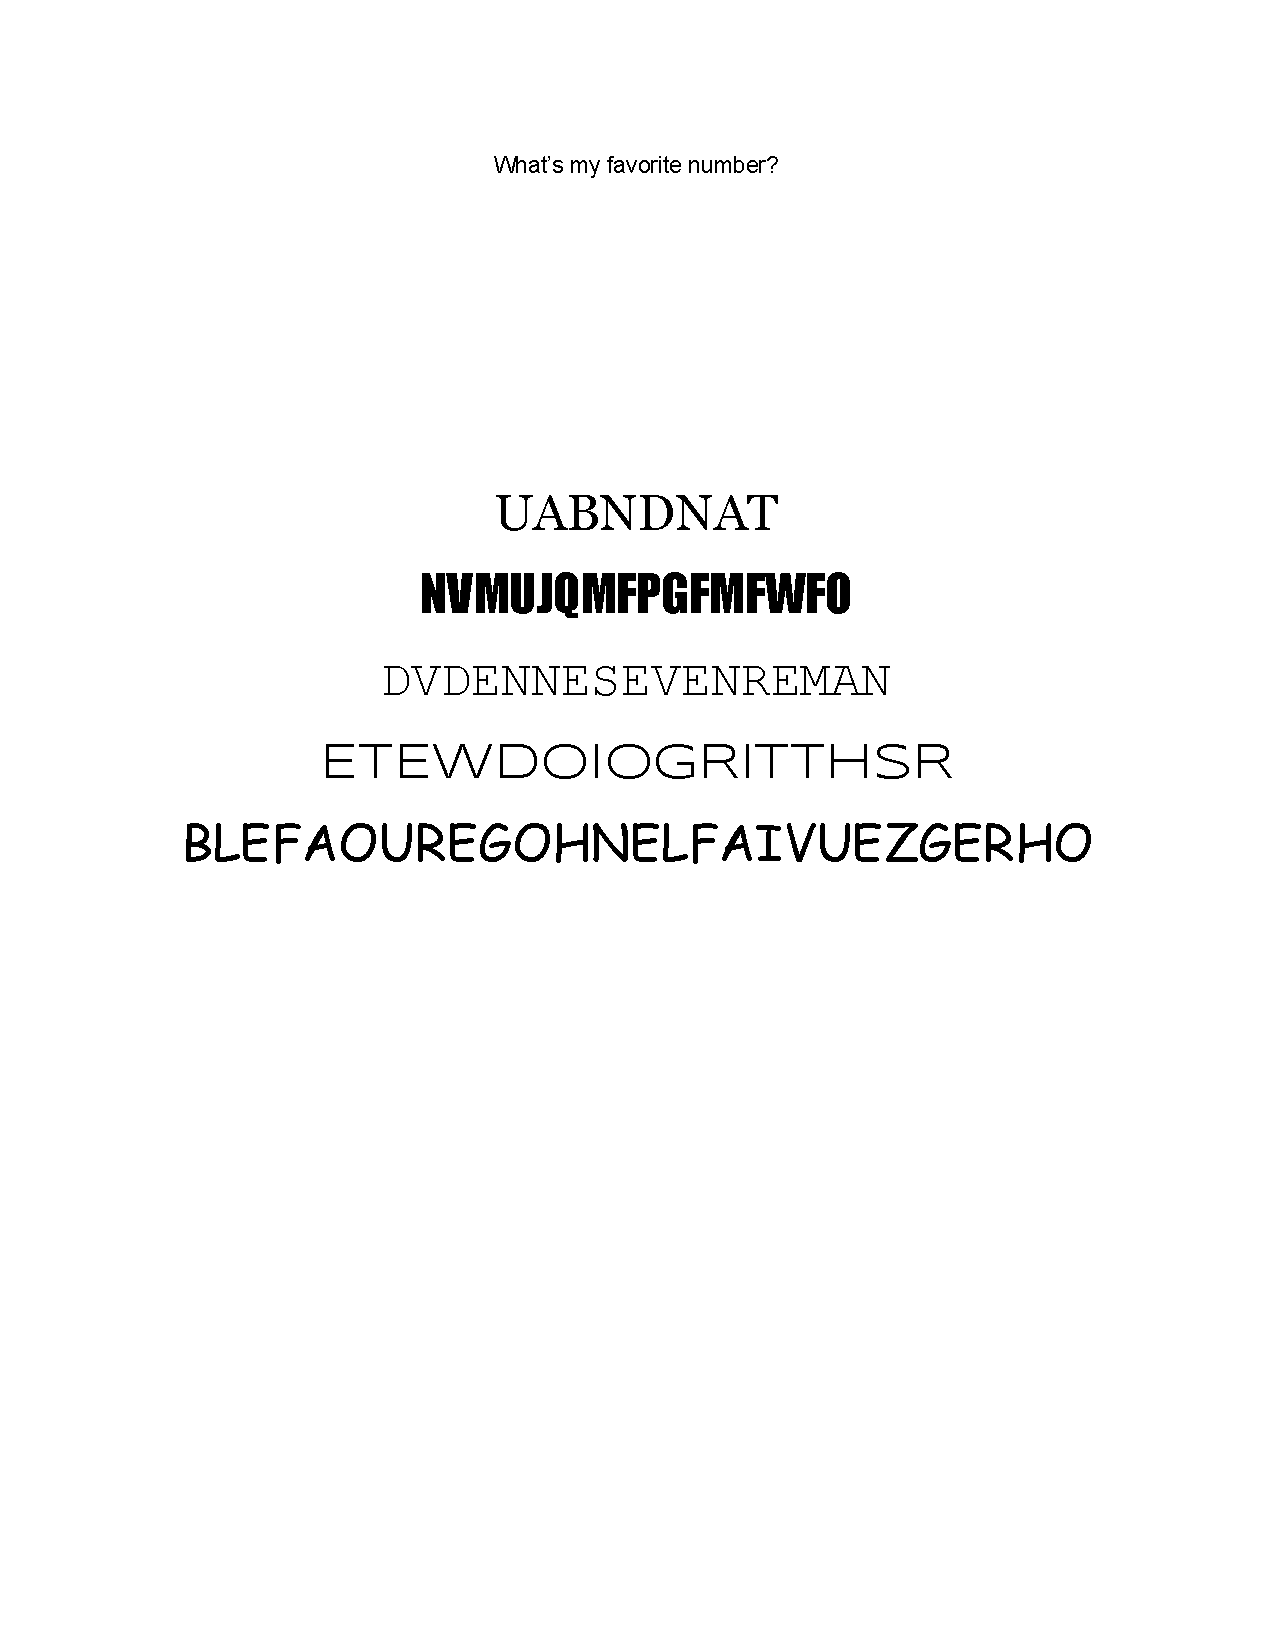
\includepdf[pages=1]{metapuzzle-page.pdf}

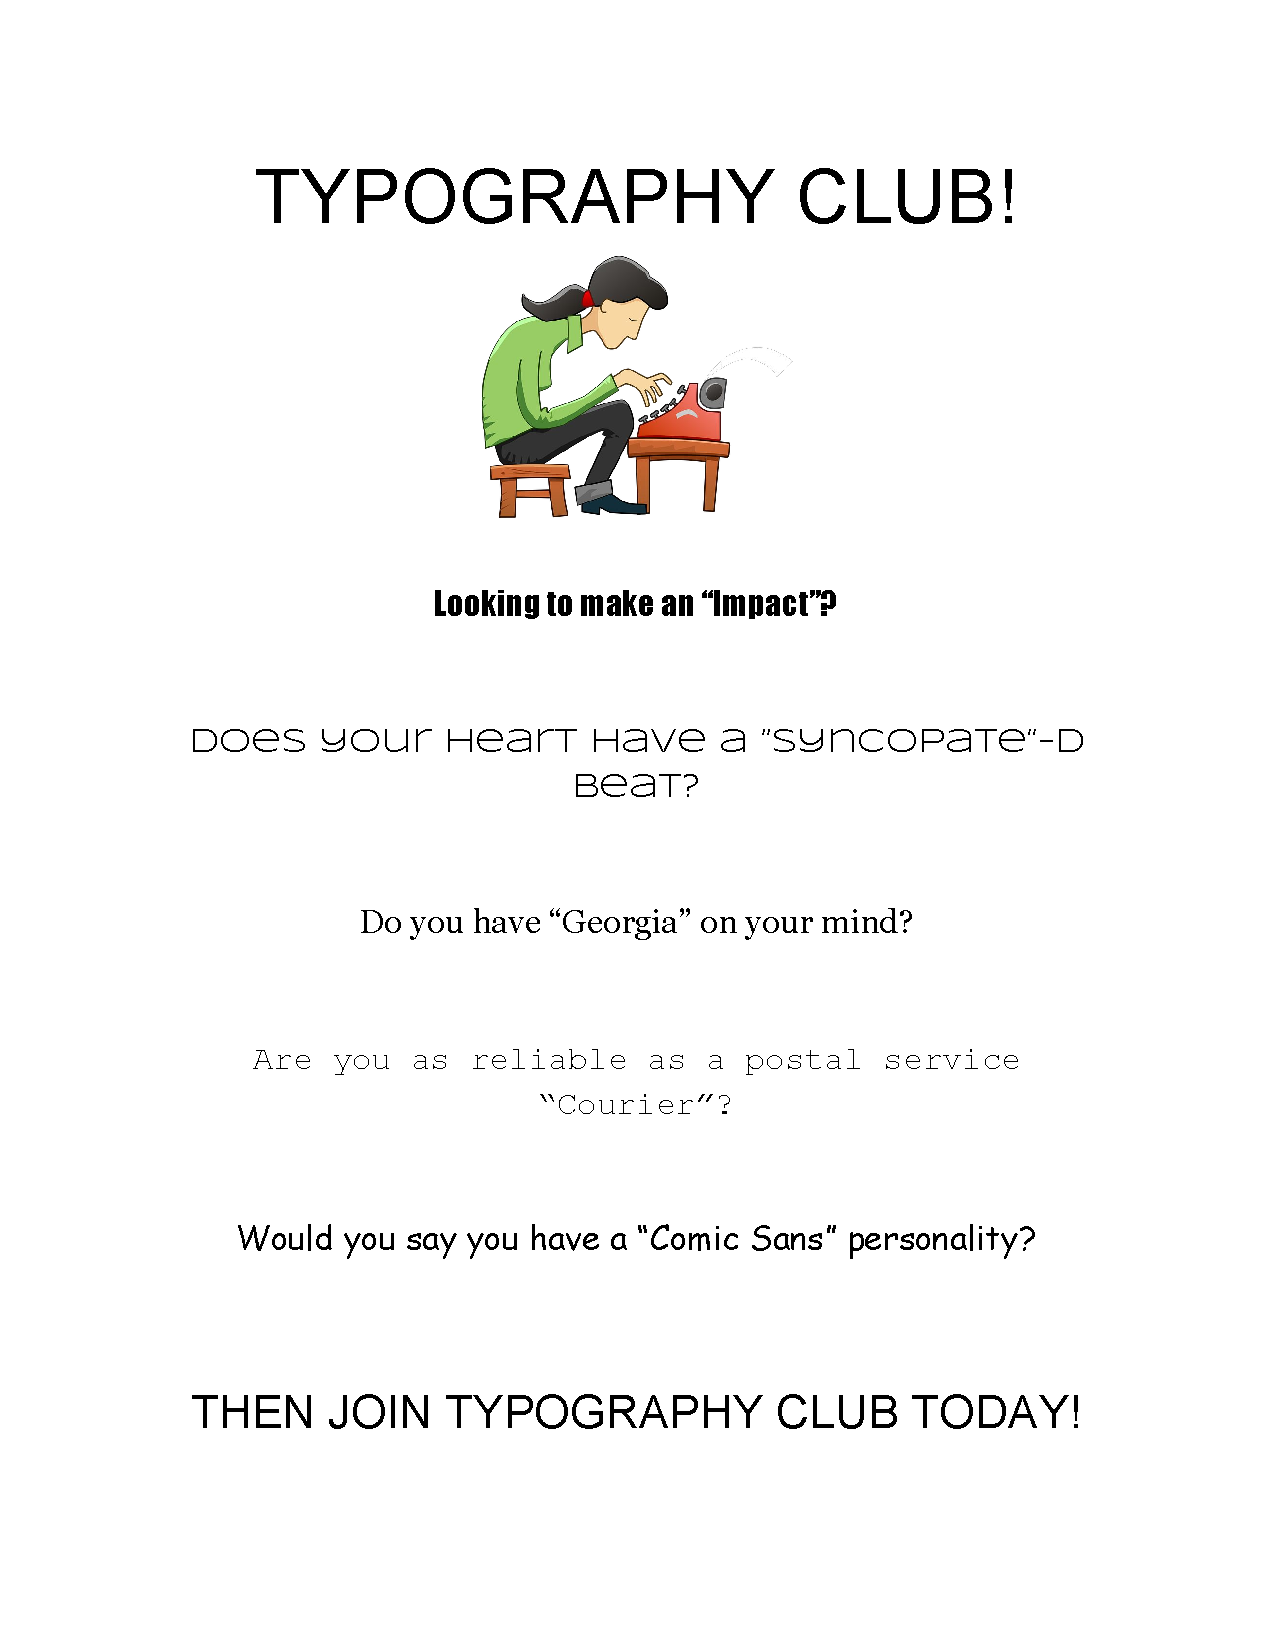
\includepdf[pages=1]{typography-club.pdf}
